
\documentclass[10pt, conference, compsocconf]{IEEEtran}



\usepackage{cite}
\usepackage{amsmath,amssymb,amsfonts}
\usepackage{algorithmic}
\usepackage{graphicx}
\usepackage{textcomp}
\usepackage{float}
\usepackage{url}
\usepackage{listings}

\usepackage{colortbl}
%\usepackage{multirow}
%\usepackage{booktabs}



\definecolor{CEWebSHeading}{cmyk}{0,0,0,0.13}
\definecolor{CEWebSImportant}{cmyk}{0,0,0,0.05}
\definecolor{CEWebSUrgent}{cmyk}{0,1,1,0.13}
\definecolor{CEWebSBad}{cmyk}{0,0.25,0.25,0}
\definecolor{CEWebSGood}{cmyk}{0.25,0,0.25,0}
\definecolor{CEWebSNeutral}{cmyk}{0.25,0.25,0,0}

\definecolor{white}{rgb}{1.0,1.0,1.0}
\definecolor{black}{rgb}{0.0,0.0,0.0}

\definecolor{darkblue}{rgb}{0.0,0.0,0.6}
\definecolor{darkred}{rgb}{0.6,0.0,0.0}
\definecolor{darkgreen}{rgb}{0.0,0.6,0.0}
\definecolor{light-gray}{rgb}{0.95,0.95,0.95}

\lstloadlanguages{ XML, SQL, Java, bash, Ant }
\lstset{
		language=XML,
    backgroundcolor=\color{light-gray},		
    basicstyle=\ttfamily\scriptsize\color{black},
%    commentstyle=\itshape\color{darkgreen}, %tiny, scriptsize
%    keywordstyle=\bfseries\color{darkblue},
%    stringstyle=\color{darkblue},  		
%    frameround=fttt,
%    frame=trBL,
%    float=hbtp,
    frame=single,
    framerule=0.4pt,
		numbers=none,
    columns=fixed,
    numberstyle=\tiny,
		extendedchars=true,
    columns=flexible,
    tabsize=2,
    showspaces=false,
    showstringspaces=false,
    breaklines=true,
    breakautoindent=true,
    captionpos=b
}

\def\BibTeX{{\rm B\kern-.05em{\sc i\kern-.025em b}\kern-.08em
    T\kern-.1667em\lower.7ex\hbox{E}\kern-.125emX}}

% correct bad hyphenation here
\hyphenation{op-tical net-works semi-conduc-tor}


\begin{document}

\title{XXX titile}


\author{
\IEEEauthorblockN{Aliaksandr Adamenko}
\IEEEauthorblockA{\textit{University of Vienna} \\
Vienna, Austria \\
alexadamenko@gmail.com}
\and
\IEEEauthorblockN{Andrii Fedorenko}
\IEEEauthorblockA{\textit{University of Vienna} \\
Vienna, Austria \\
andriifedorenko@gmail.com}
\and
\IEEEauthorblockN{Erich Schikuta}
\IEEEauthorblockA{\textit{University of Vienna} \\
Vienna, Austria \\
erich.schikuta@univie.ac.at}
}


\maketitle


\begin{abstract}
XXXXX

\end{abstract}

\begin{IEEEkeywords}
xxx; xxxx;

\end{IEEEkeywords}



\IEEEpeerreviewmaketitle



\section{Introduction}
XXX


\section{Related Work and Baseline Research}

XXX


\section{N2Sky Architecture}
\label{N2Sky Architecture}

N2Sky is a simulation platform, which allows all involved stockholders to use it for computational purposes. In order to achieve high performance and scalability, it was decided to use the microservices architecture. This approach is used not only on backend services, but also with frontend and its services. 






\section{User-centered Interface within modular frontend}
\label{User-centered Interface within modular frontend}

The basis of N2Sky is the user-centered design. Moving from complex monolithic application to easily understandable one we were concentrated on past user experianses. To gain the functionality and increase the performance of the application were a fundamental requirement. 

\label{modular_frontend}
\subsection{User Role as an Independent User Interface}
\label{User Role as an Independent User Interface}
N2Sky web, as well as the mobile portal, has an intuitive user interface. Since N2Sky is an expert for different knowledge level users it was decided to separate the user roles. Every user namely user role has its own user interface, which is deeply integrated with user needs. The professionals will get detailed information about processes with a technical jargon, simple arbitrary users will get more simplified information. 

\begin{itemize}
\item \emph{Arbitrary User.}  The Arbitrary User a user, who does not have a deep knowledge of the neural network field or know any programming language. His main purpose is not a contribution, but the usage already existing neural networks and trained models. The main goal of the arbitrary user is to study neural networks within N2Sky platform. The arbitrary user can also evaluate the trained models or execute training against existing neural networks. This kind of user does not have to use his own training data, he just wants to see the behavior of neural networks. The arbitrary user can be converted to Neural Network Engineer user if he has enough knowledge of it. 
\item \emph{Neural Network Engineer.} The Neural Network Engineer is an arbitrary user. The Neural Network Engineer has an access only to his own dashboard and publicly available resources on the main application module. He can perform the semantic search for available neural network paradigms and use them. This user can create own neural network instance from existing neural network paradigm. He can also train the running neural network instances and evaluate their trained models. This user can share his trained neural network by making it public. 
\item \emph{Contributor.} The Contributor is an expert user, which has enough knowledge and experience to create his own neural network. This user can create neural network paradigms using the ViNNSL template schema \cite{Beran2008} and publish them on N2Sky. This user can deploy neural networks on the N2Sky environment as well as on his own environment by providing training and testing endpoints. The goal of the contributor is the study how his networks will behave with different network structures, input parameters and training data that is provided by other users.
\item \emph{System Administrator.} System Administrator is a user who has a full access to the application including environment management, monitoring and alerting features. The administrator can manage OpenStack and Cloudify instances. He also can shadow any N2Sky user to observe the application from other perspectives. The administrator has access to all dashboards in every module.
\end{itemize}



\subsection{Modular frontend application design}
\label{Modular frontend application design}

Maintain the large application like N2Sky with the monolithic approach is unwieldy. Since N2Sky supports microservices approach in the backend it was decided to apply the same solution on the frontend.  

Microservices in frontend are small independent web applications, which are consolidated into one application. The main benefits of this approach are:


\begin{itemize}
\item \emph{Maintainability.} It is possible to divide application between different teams. Developers do not even need to have some knowledge about other parts of the application. 
\item \emph{Diversity of technologies.} Monolithic approach makes the whole application stick to one framework. Microservices allowing to use any technology without the need to rewriting the application.
\item \emph{Independent deployment.} Every application has some releases periods, every release accompanies with redeployment procedure. There is no need to redeploy the whole application, but just only required components.
\end{itemize}

\begin{figure}[H]
  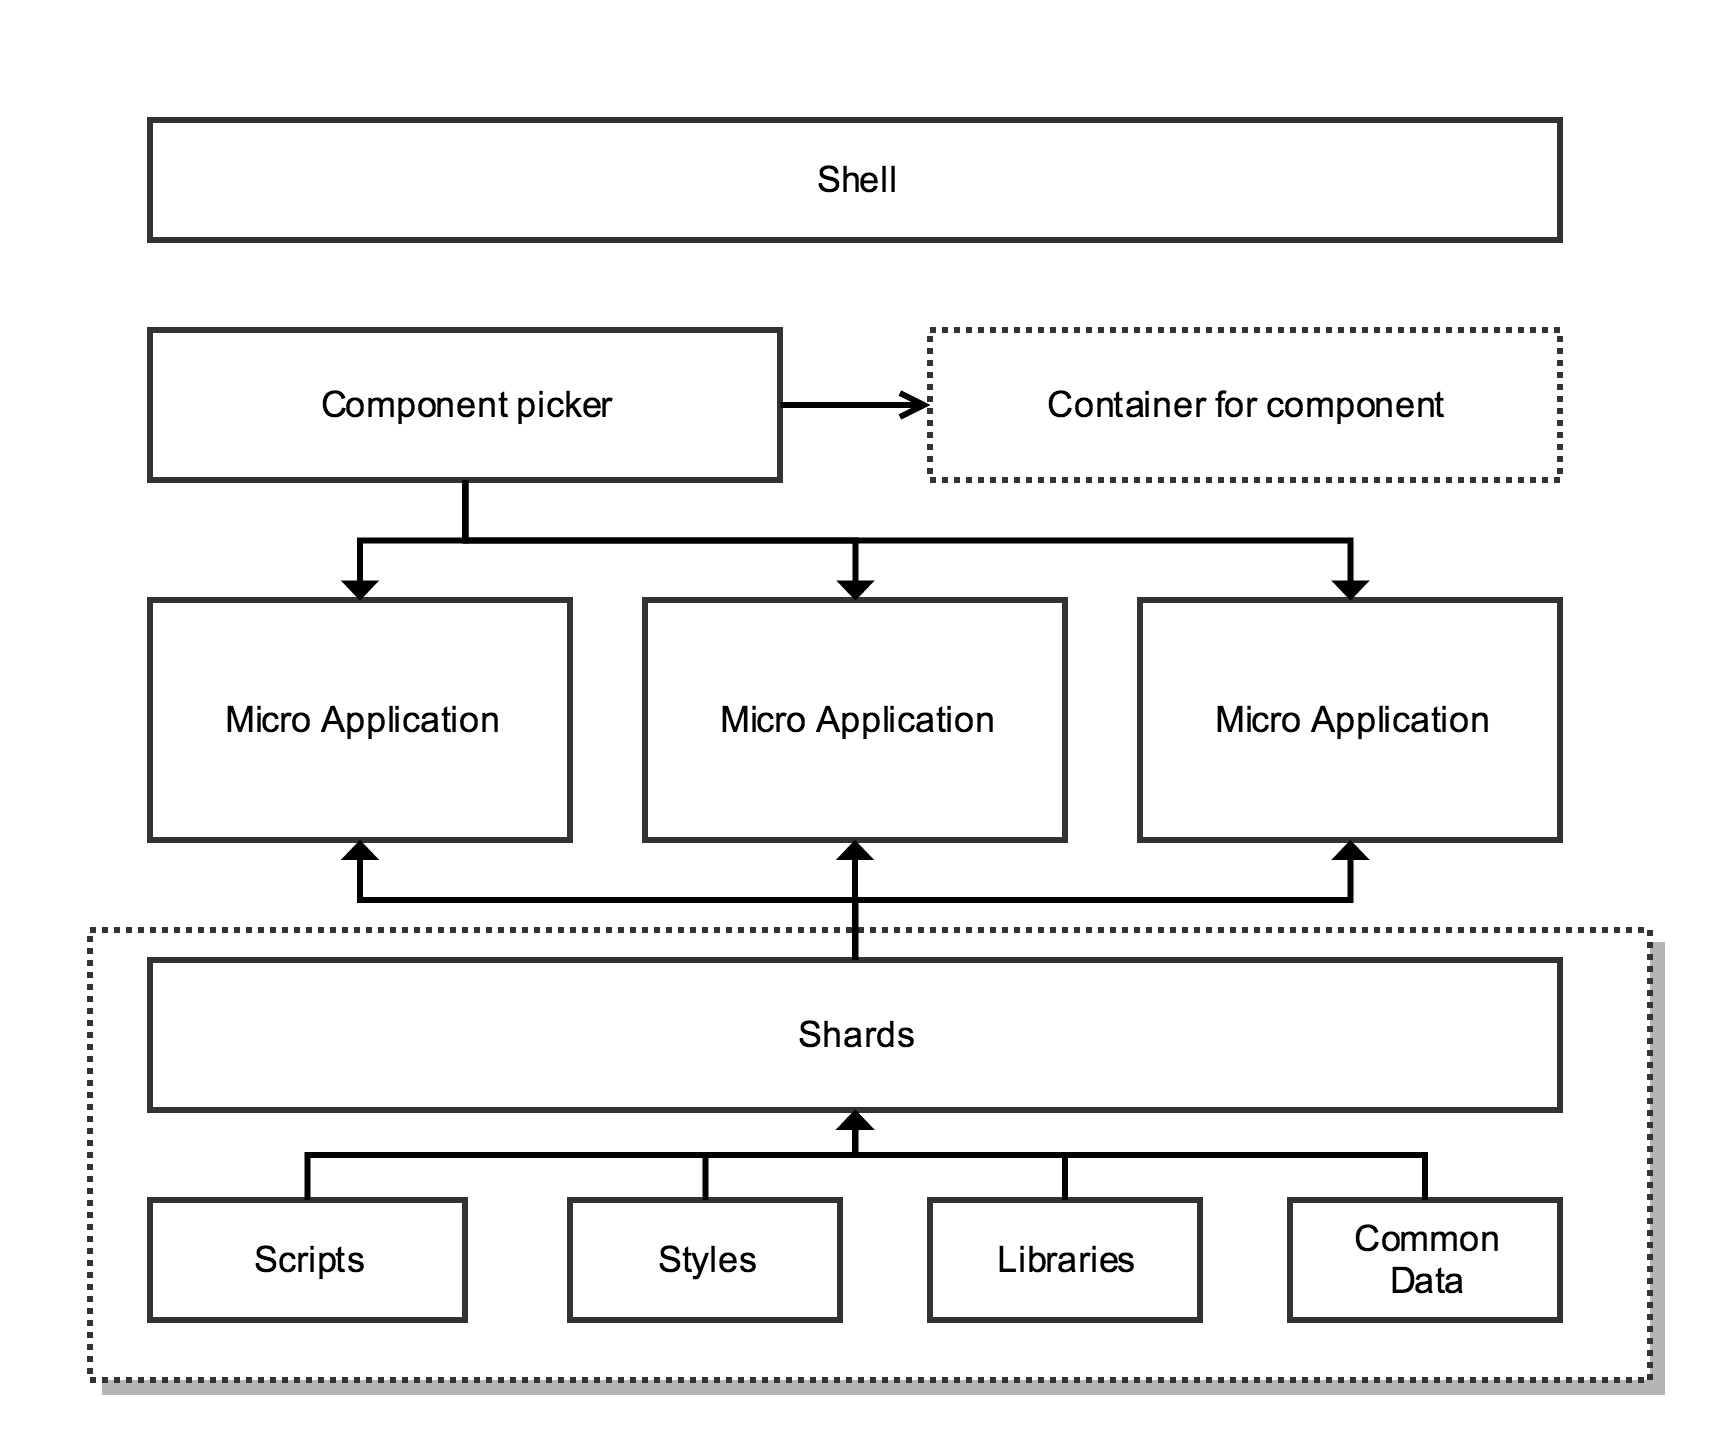
\includegraphics[width=\linewidth]{img/frontend_arch.png}
  \caption{Microservices approach in frontend application}
  \label{fig:frontend_arch}
\end{figure}

Microservices approach in frontend application is shown in ``Fig.~\ref{fig:frontend_arch}''. This breaks the entire application into small micro applications \cite{frontendMicro}.

\begin{itemize}
\item \emph{Shell.}  is a top-level component, which wraps Components picker and Container for the component. It contains application configuration.
\item \emph{Component picker.} Is a router, which manages the micro applications. 
\item \emph{Container for Component.} Container, where the component will be injected.
\item \emph{Micro Application.} Independent application, which can be written in any programming language but has to use one of the shards.
\item \emph{Shards.} Is a code base, which is shared between Micro Applications. Shards can have multiple levels. 
\end{itemize}
 
\subsection{N2Sky modular frontend}
\label{N2Sky modular frontend}

The central concept of the application is to support the Software as a Service (SaaS) and Platform as a Service (PaaS) distributions \cite{Walraven2014}.  N2Sky consists of two modules: administration module, main application module as it shown in ``Fig.~\ref{fig:modular_design}''.



\begin{figure}[H]
  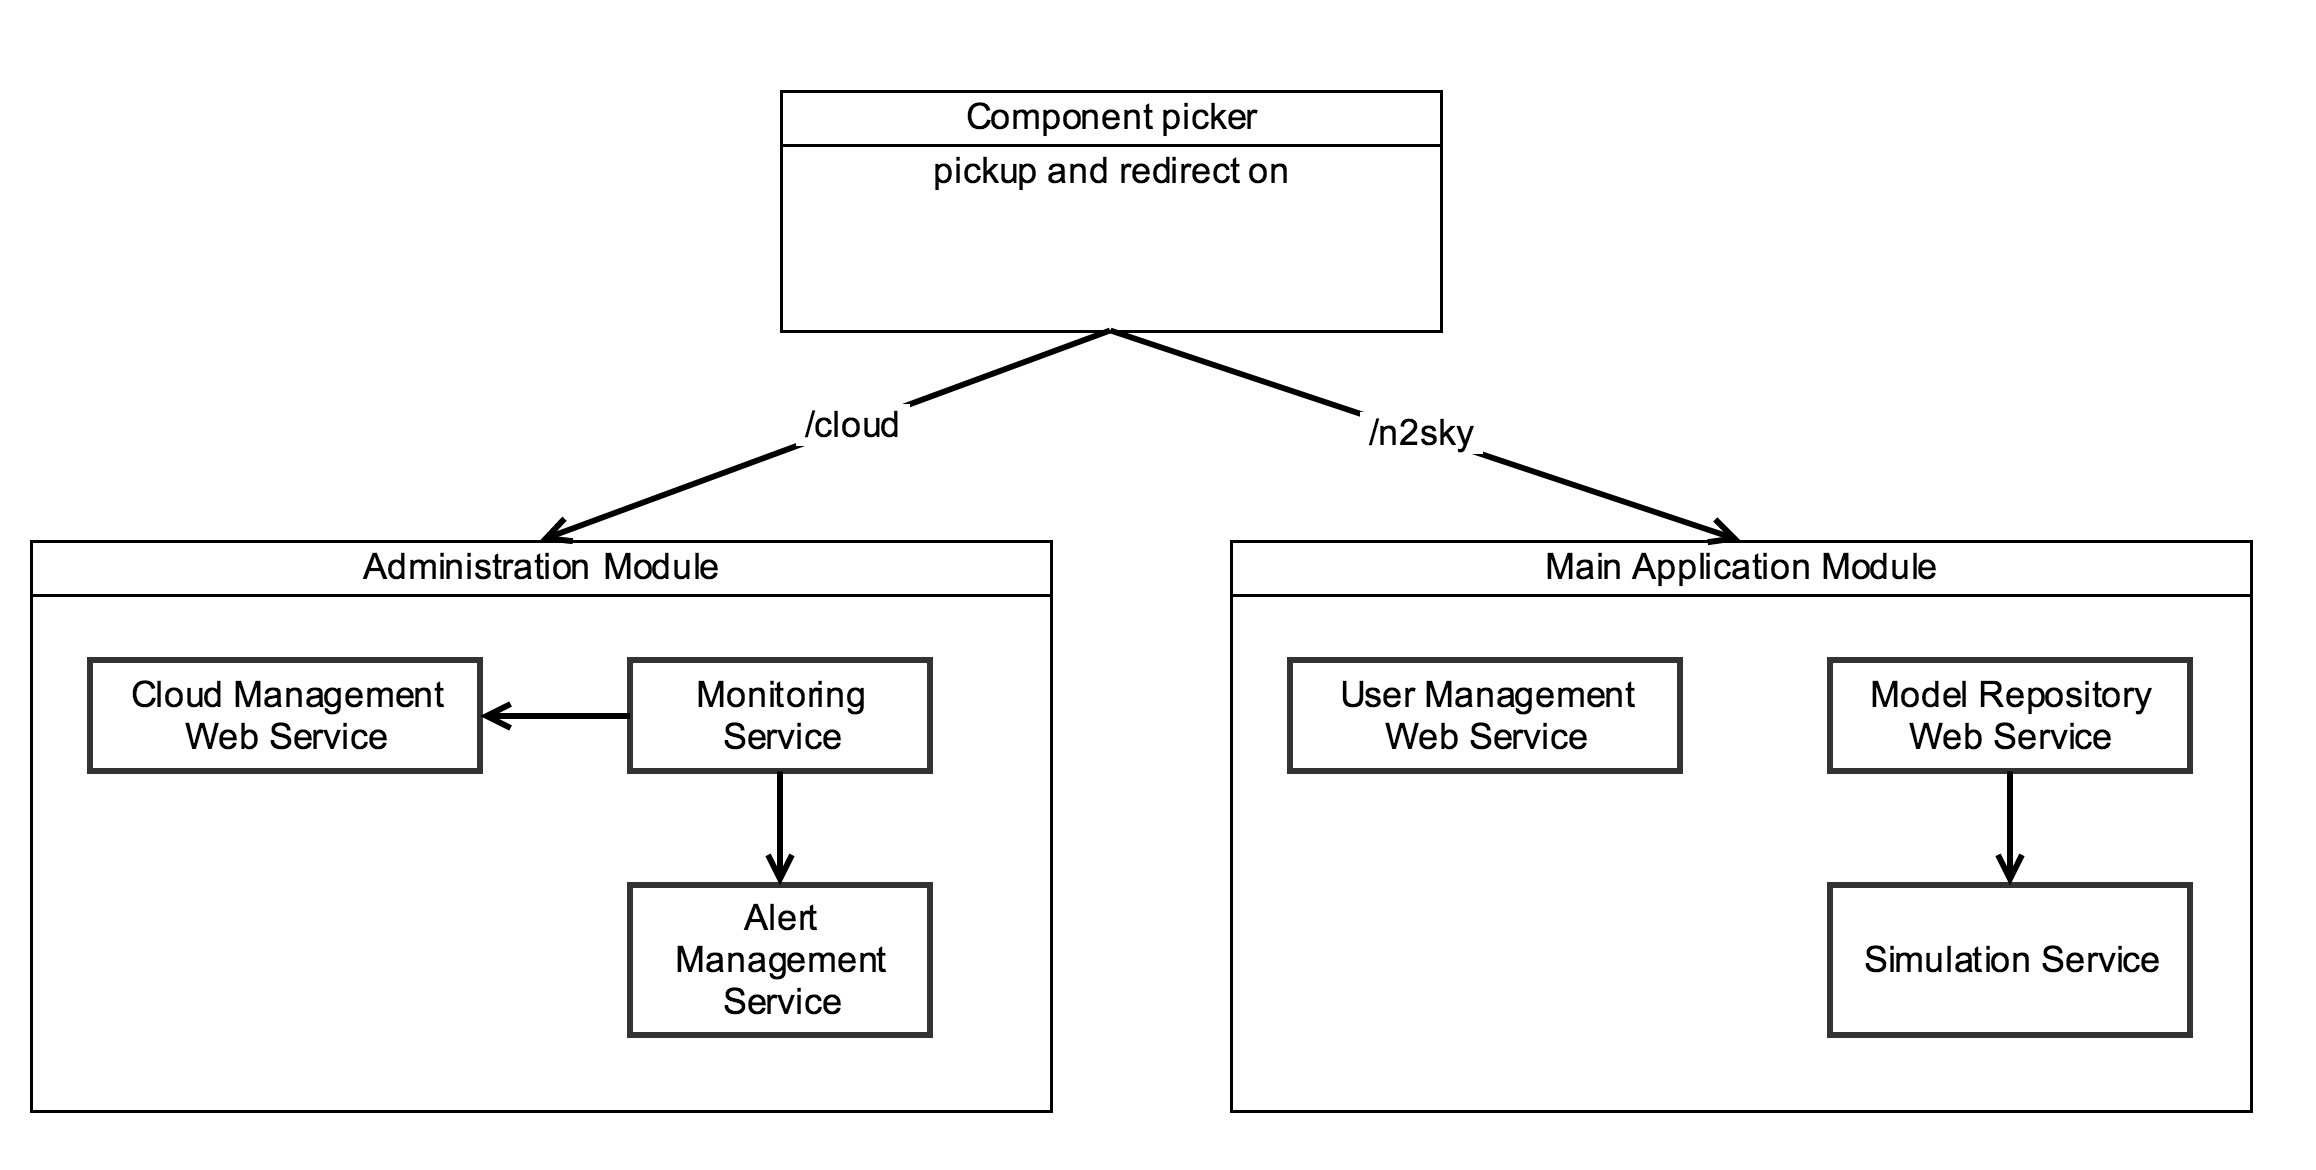
\includegraphics[width=\linewidth]{img/redirector.png}
  \caption{N2Sky frontend application and its services}
  \label{fig:modular_design}
\end{figure}


\begin{itemize}
\item \emph{N2Sky component picker.} When the user goes to N2Sky web portal, first he will be dealing with a component picker. The component picker is a small service, which redirects the user depending on URL path.
\begin{itemize}
\item \emph{/cloud} redirects to "Administration module"
\item \emph{/n2sky} redirects to "Main application module"
\end{itemize}

\item \emph{Administration module} The administration module allows the system administrator to control the environment. The module supports OpenStack and Cloudify monitoring. Managing is possible through the application dashboard. It also contains custom monitoring and an alerting management system, which can be installed on any server within the N2Sky user interface. The administration module implements PaaS. It is fully configurable and wrapped into the open source project in order to make the module accessible to the third-party applications. 
\item \emph{Main application module} The main application module is the central module of N2Sky. Within this module, users can use, train and test existing neural networks. It is possible to reuse the neural network paradigms and create own neural network. N2Sky allows deploying own network and store data in the cloud. Module services are supporting the SaaS distribution. Experts can use an application directly through the N2Sky API or they can integrate N2Sky services into their own application. 
\end{itemize}

\section{The sample workflow}


To support Software as a Service (SaaS) distribution every web service can work independently. It means that the stakeholders can use N2Sky via web portal as well as use N2Sky API.
N2Sky API allows  stakeholders:

\begin{itemize}
\item Authorise in the System
\item Create new neural from existing paradigm
\item Deploy own neural network on N2Sky environment 
\item Perform training against own as well published neural network
\item Perform testing against trained models
\end{itemize}


\begin{figure}[H]
  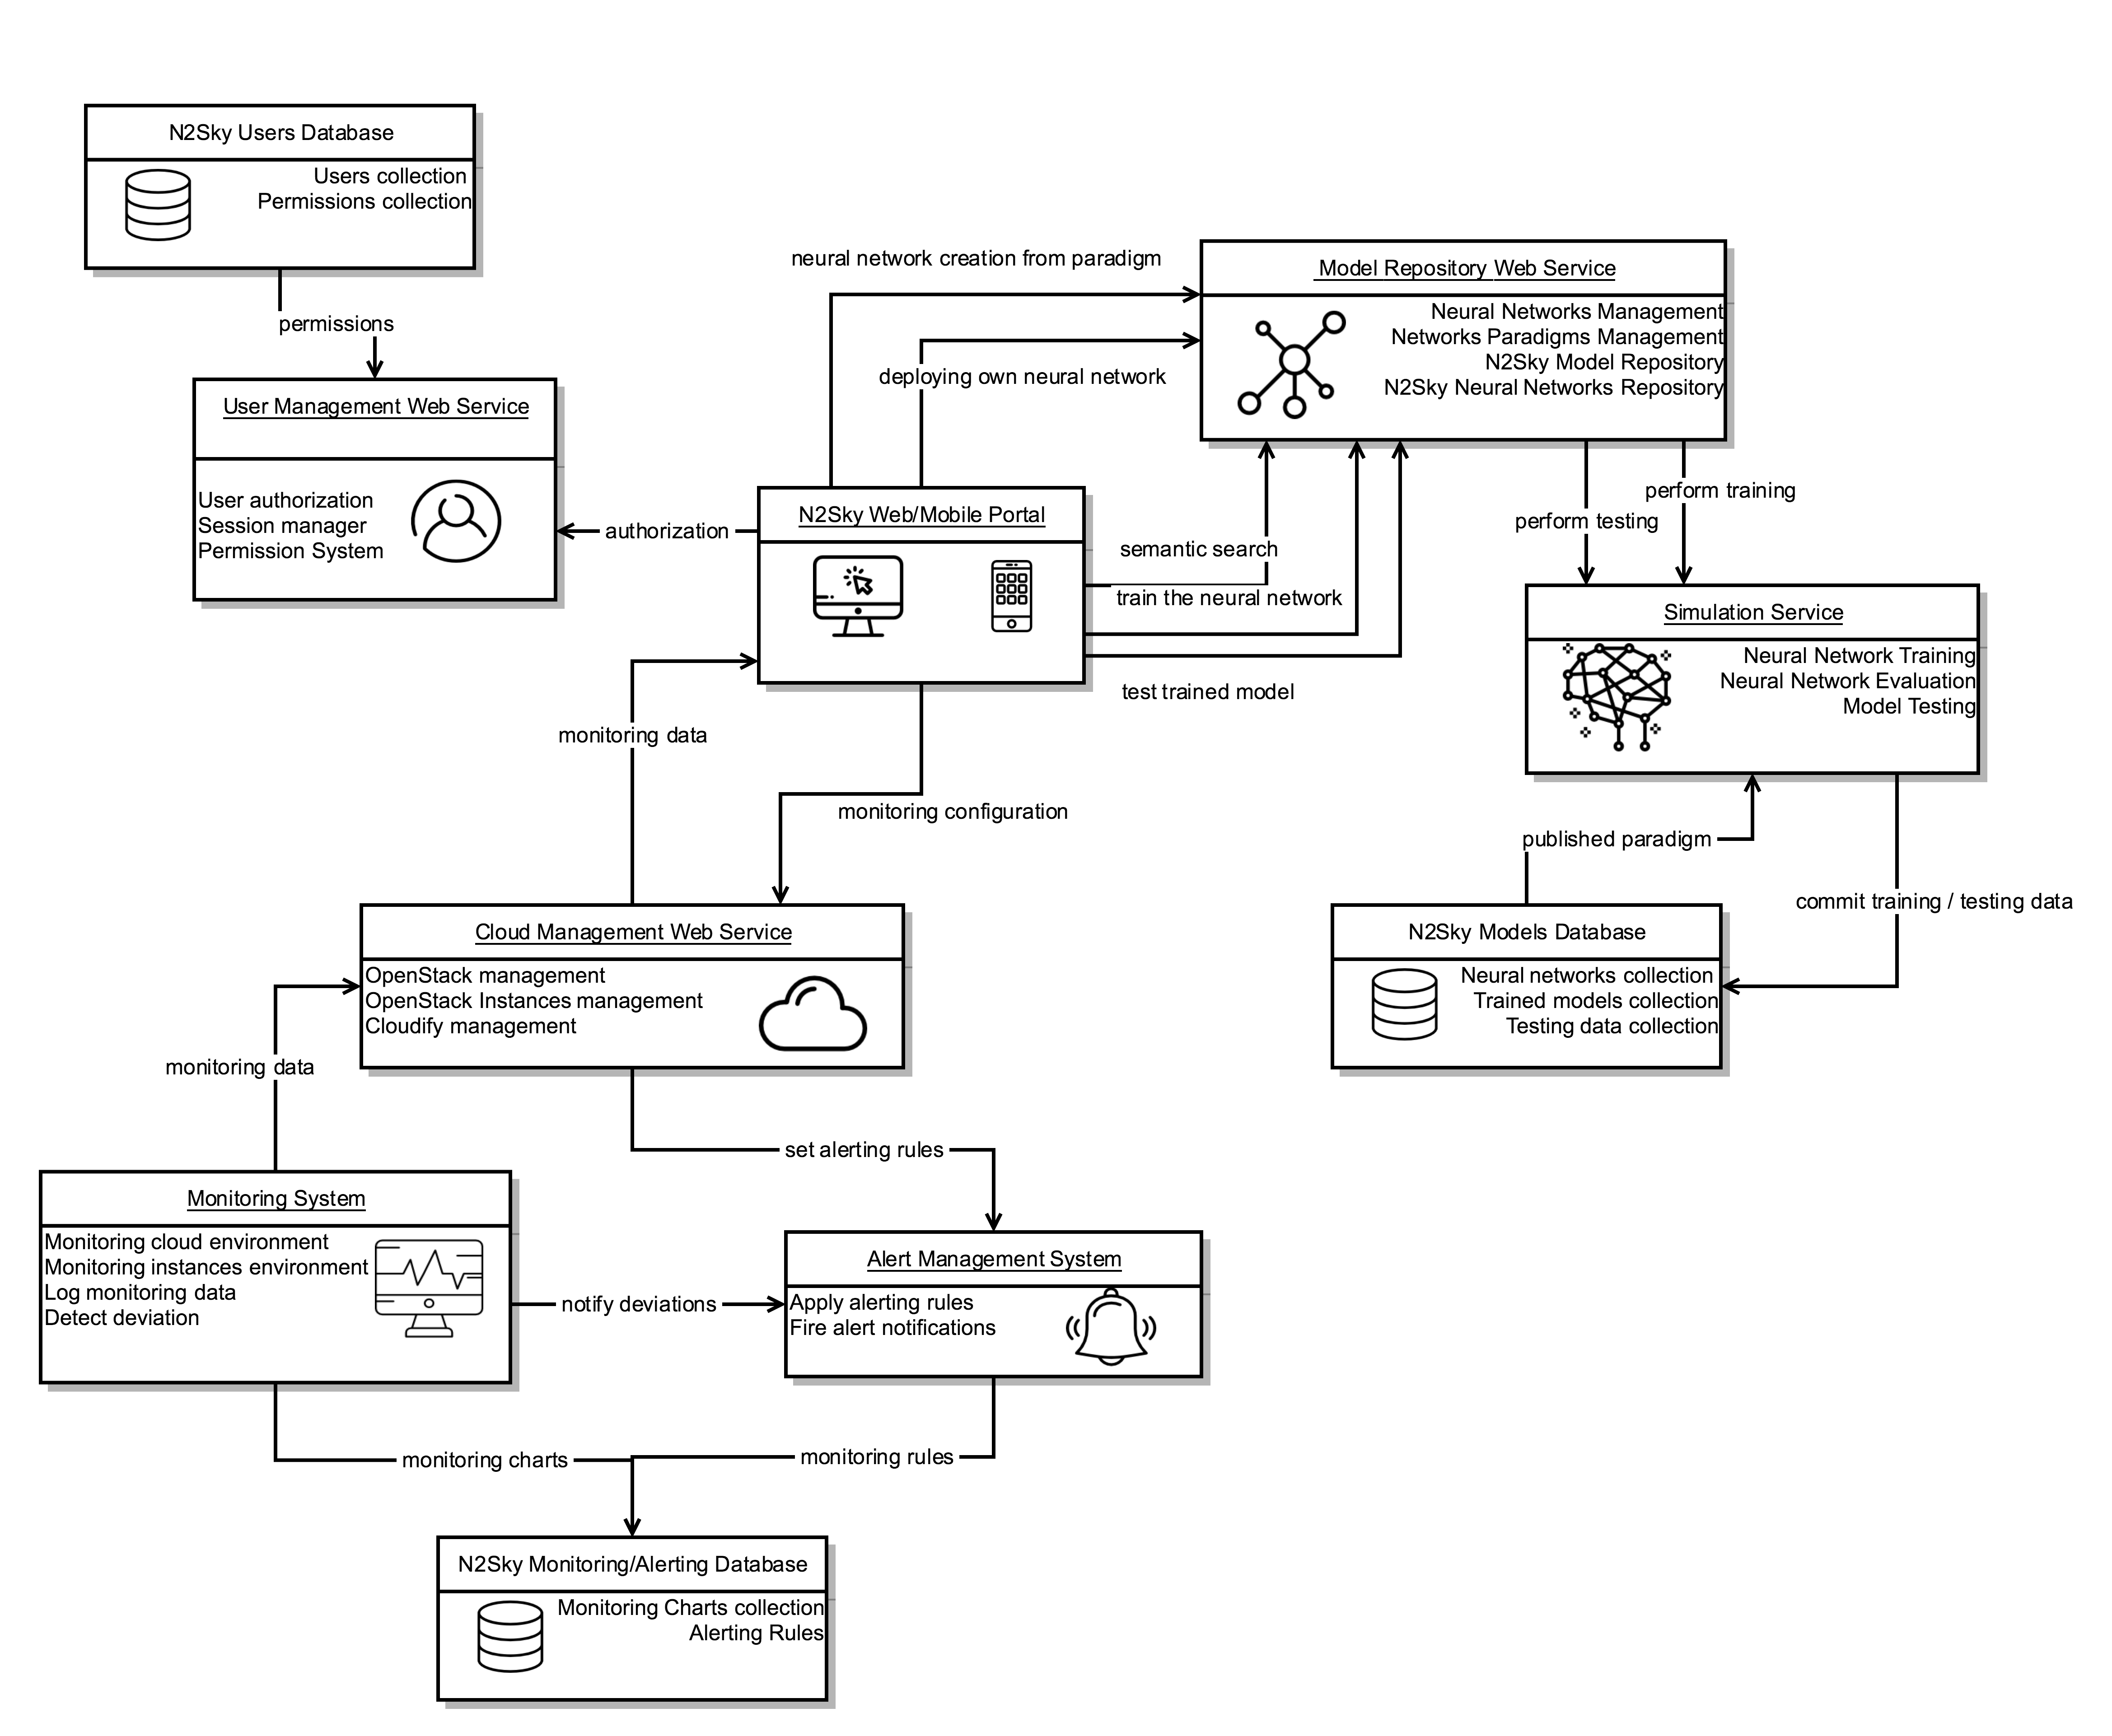
\includegraphics[width=\linewidth]{img/new_arch.png}
  \caption{The sample workflow}
  \label{fig:newarch}
\end{figure}



The sample workflow overview, which shown in figure~\ref{fig:newarch} represents microservices architecture in action:


\begin{enumerate}
\item \emph{Contributor User}
\begin{enumerate}
\item The Contributor user authorize in the N2Sky portal using his browser on desktop PC or mobile device. He will be redirected to his own dashboard according to permissions, which will be received from User Management Web Service. 
\item The user described his own neural network paradigm using the ViNNSL template and deploying it in the N2Sky cloud as it shown in ~\ref{fig:own_nn}. 

\begin{figure}[H]
  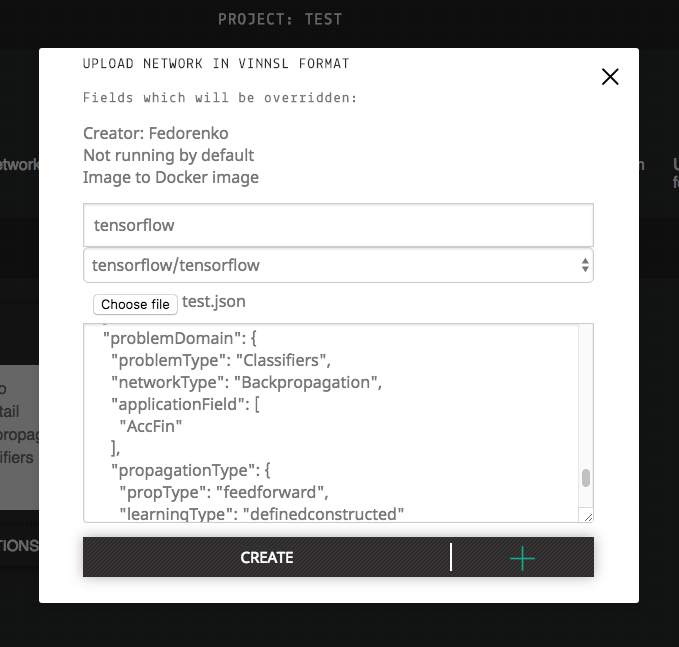
\includegraphics[width=\linewidth]{img/own_nn.png}
  \caption{The user uploads the neural network paradigm description in ViNNSL format}
  \label{fig:own_nn}
\end{figure}

\item The Contributor user perform training of his neural network using the N2Sky platform. Since the user is an expert he can perform this operation using Simulation Service via Model Repository Web Service API.
\item The user publishes his paradigm via N2Sky UI or available API. 
\item The Contributor user awaiting until other N2Sky users will use his neural network paradigm in order to monitor the behavior of the neural network. 
\item The user modify, redeploy and retrain his neural network after first results. 
\end{enumerate}
\item \emph{Neural Network Engineer User}
\begin{enumerate}
\item The neural network engineer user authorize in the N2Sky portal using his browser on desktop PC or mobile device. He will be redirected to his own dashboard according to permissions, which will be received from User Management Web Service. 
\item From the dashboard, the user creates a neural network from existing paradigm using Model Repository Web Service. The user specify the neural network structure as it shown in ~\ref{fig:structure}.


\begin{figure}[H]
  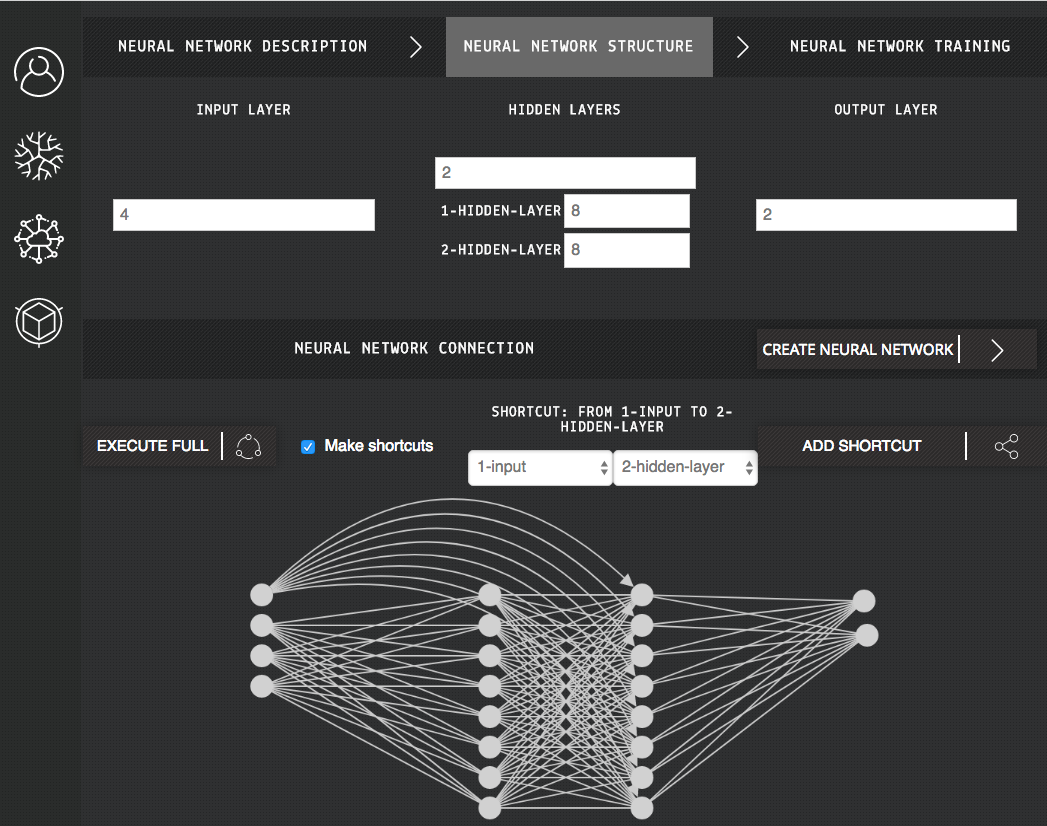
\includegraphics[width=\linewidth]{img/structure.png}
  \caption{The user specifies the neural network structure}
  \label{fig:structure}
\end{figure}

 
\item The user perform training against his newly created neural network using the N2Sky platform as it shown in ~\ref{fig:eval}. 

\begin{figure}[H]
  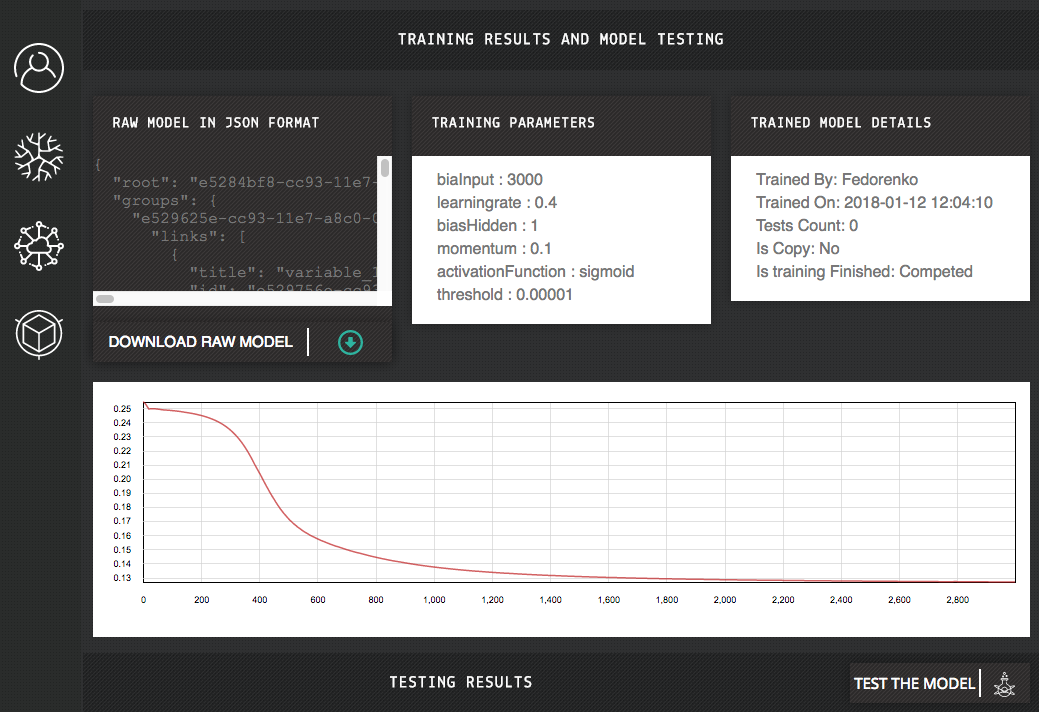
\includegraphics[width=\linewidth]{img/eval.png}
  \caption{The user performs neural network training}
  \label{fig:eval}
\end{figure}


\item If the user satisfied with a trained model he can perform testing using the N2Sky platform. 
\item The neural network engineer user publish his neural network and trained model in order to make it available for other N2Sky users. 
\end{enumerate}
\item \emph{Arbitrary User}
\begin{enumerate}
\item The arbitrary user authorize in the N2Sky portal using his browser on desktop PC or mobile device. He will be redirected to his own dashboard according to permissions, which will be received from User Management Web Service. 
\item Since the user does not much knowledge in neural network field, he performs a semantic search in order to find some neural network as well as trained models according to his needs as it shown in ~\ref{fig:repo}. 

\begin{figure}[H]
  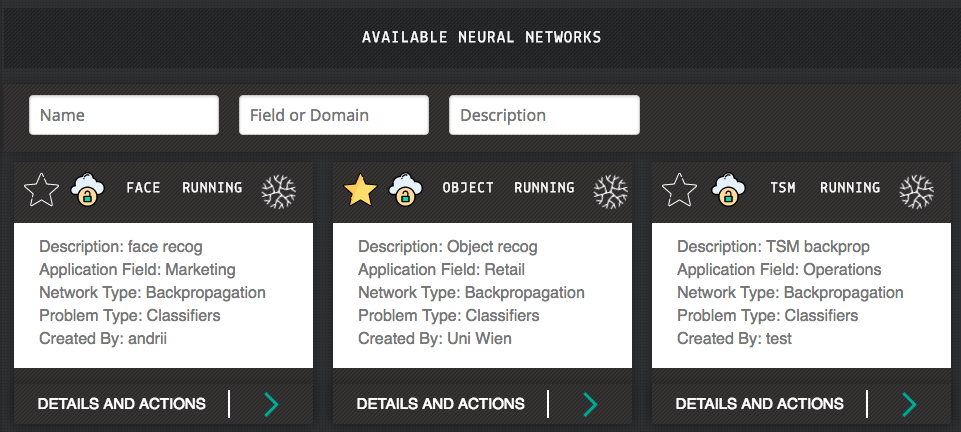
\includegraphics[width=\linewidth]{img/repo.png}
  \caption{The user performs semantic search in Neural Network Repository}
  \label{fig:repo}
\end{figure}


\item The user copy existing neural network and some trained models into his project. 
\item The user perform training from N2Sky platform against copied neural network with the default input parameters data.
\item The user evaluate trained neural network model with the default parameters. 
\end{enumerate}
\item \emph{System Administrator}
\begin{enumerate}
\item The system administrator authorize in the N2Sky portal using his browser on desktop PC or mobile device. He will be redirected to administration dashboard.
\item The user observes cloud environment.
\item The system administrator creates the new monitoring chart with a specific metrics and add it to the administration dashboard.
\item The user creates alert against newly created monitoring
\item The user is notified by Alert Management System, that some event occurs.
\end{enumerate}
\end{enumerate}




\section{Conclusion}
The conclusion goes here. this is more of the conclusion

% conference papers do not normally have an appendix


% use section* for acknowledgement
\section*{Acknowledgment}


The authors would like to thank...
more thanks here


% trigger a \newpage just before the given reference
% number - used to balance the columns on the last page
% adjust value as needed - may need to be readjusted if
% the document is modified later
%\IEEEtriggeratref{8}
% The "triggered" command can be changed if desired:
%\IEEEtriggercmd{\enlargethispage{-5in}}

% references section

% can use a bibliography generated by BibTeX as a .bbl file
% BibTeX documentation can be easily obtained at:
% http://www.ctan.org/tex-archive/biblio/bibtex/contrib/doc/
% The IEEEtran BibTeX style support page is at:
% http://www.michaelshell.org/tex/ieeetran/bibtex/
%\bibliographystyle{IEEEtran}
% argument is your BibTeX string definitions and bibliography database(s)
%\bibliography{IEEEabrv,../bib/paper}
%
% <OR> manually copy in the resultant .bbl file
% set second argument of \begin to the number of references
% (used to reserve space for the reference number labels box)

\bibliographystyle{plain}
\bibliography{bibliography}


% that's all folks
\end{document}


